
\chapter{General Background and Fundamental Concepts}
\label{chapter:general-background}

This chapter presents the general background and fundamental concepts related to the domain problem that is addressed in this thesis.
At the first section (\autoref{sec:cscl-and-scripted-collaboration}), an overview of the CSCL field and scripted collaborative learning is presented to provide a comprehensive and elucidate accord about the research context.
This section also describes in detail the motivational problems in scripted collaborative learning, as well as, the current approaches to deal with them.
The \autoref{sec:gamification} presents an overview of gamification, and the theoretical foundation of this technology.
%This section also presents a briefly revision of research works that have realized in gamification in the context of CSCL and other educational contexts.
Finally, \autoref{sec:ontologies-and-ontology-engineering} presents the fundamentals of ontologies and ontology engineering.
%This sections also discusses how ontologies and ontology engineering is currently used to support the systematic formalization of theory-based knowledge, and how this formalization currently help us to overcome some problems in the field of Artificial Intelligence in Education.

%% ================================== %%

\section{CSCL and Scripted Collaborative Learning}
\label{sec:cscl-and-scripted-collaboration}

Although CL has a long history in education, it is not until the early 1990s that the research field known as Computer-Supported Collaborative Learning (CSCL) had gained attention and strength \cite{StahlKoschmannSuthers2006}.
CSCL is the field dedicated to study how to provide support for CL through computational technology and Internet.
This research field is a multidisciplinary field that combines studies from the Cognitive Psychology Education and from the Computer Science to effectively enhance the CL process \cite{HoppeOgataSoller2007}.

The general aim of CSCL field is to develop technologies to support or create situations in which two or more students learn together through the interaction among them \cite{Dillenbourg1999}.
In these situations, the learning outcomes are a consequence of students' interactions and how these interactions affect the individual learning for each one of the students.
Therefore, to enable a well-though-out design of CL, the CSCL scripts have been proposed by the CSCL community as the technology to facilitate the social and cognitive processes of learning by delineating the way in which the learners will interact with each other in a CL scenario \cite{HarrerKobbeMalzahn2007}.

\subsection{CSCL Scripts}
\label{sec:cscl-scripts}

CSCL scripts are the technology that describes the way of student should collaborate to achieve positive learning outcomes.
These scripts basically structure and orchestrate the CL process to attain pedagogical objectives usually defined by an instructional design \cite{DillenbourgJermann2007}.
In this sense, the CSCL scripts are prescribed instructions that indicate how to facilitate the social and cognitive processes in group activities \cite{Dillenbourg2002}.
In order to narrow the number of elements used to describe the CSCL scripts, and provide a common and sharable description of CSCL scripts, \citeonline{KobbeWeinbergerDillenbourgHarrerHamalainenHakkinenFischer2007} propose a framework that is currently wide accepted by the community as the common specification to delineate the CSCL scripts using natural language.
This framework formalizes the CSCL scripts as a set of components and mechanisms illustrate in \autoref{fig:components-and-mechanisms-of-cscl-scripts}.


\begin{figure}[htb]
 \caption{Components and mechanisms of CSCL scripts}
 \label{fig:components-and-mechanisms-of-cscl-scripts}
 \centering
 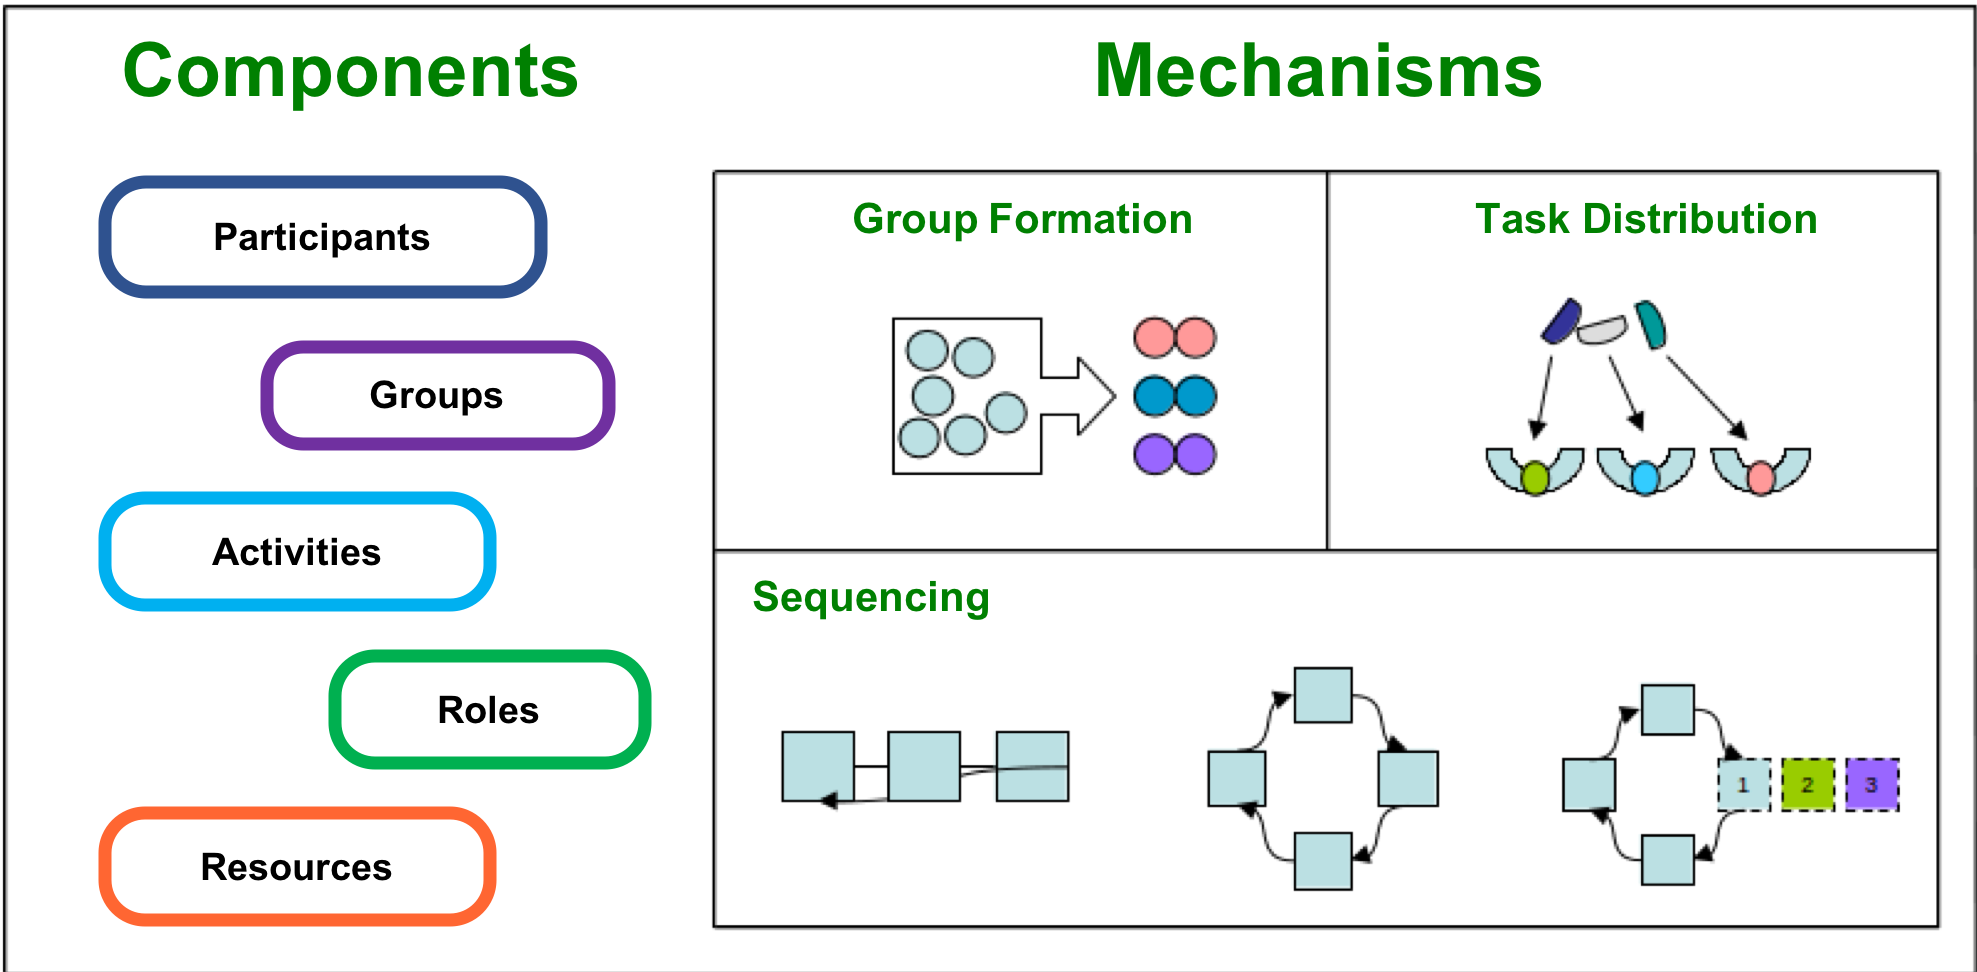
\includegraphics[width=0.95\textwidth]{images/chap-general-background/components-and-mechanisms-of-cscl-scripts}
 \fadaptada{Fischer2007}
\end{figure}

The structural \textbf{components} of CSCL scripts are the participants, groups, activities, roles and resources.
The component of \emph{participants} delineates the participants, such as learners, monitors, and teachers. 
Although this description can be abstract or concrete and simple or complex, it is often presented in a simple manner with rules that indicate conditions to participate in the CL process.
The component of \emph{activities} delineates what will be performed by the participants in the CL process to attain the learning goals defined by the instructional designers.
The component of \emph{roles} delineates the privileges, obligations and expectations of participants in the CL process.
The component of \emph{groups} of participants defines by hierarchical structures how the students are grouped according to the participants' characteristics.
The component of \emph{resources} delineates the learning objects (e.g. content resources, material, and tools) that can be used by the participants during the CL process.

The \textbf{mechanisms} of CSCL scripts are the group formation, component distribution and sequencing.
The mechanism of \emph{group formation} consists in the specifications of how the participants will be distributed over the groups in the CL process.
The mechanism of \emph{task distribution} provides the specification about how the components of scripts are distributed over groups using the mapping of groups, activities, roles, and resources.
The mechanism of \emph{sequencing} consists in the definition of how the components and groups defined in scripts are distributed over time.
In general, this sequencing delineates the interaction among the group members in the CL process.

\begin{quadro}[htb]
\caption{Components and mechanisms of social script}
\label{qua:social-script-framework-kobbe}
\centering
\footnotesize
\begin{tabular}{l p{12cm}}
\toprule
\multicolumn{2}{l}{\textbf{Structural components:}} \\ \midrule
\textbf{Participants:} &
A number of participants that must be divisible by the number of case studies.  \\
\textbf{Groups:} &
Case groups \\
\textbf{Activities:} &
(a) Applying theoretical concepts to the case study and constructing arguments \\
 &
(b) Critiquing initially scaffolder with prompts for eliciting clarification, identifying conflicting views and constructing counter-arguments \\
\textbf{Roles:} &
\emph{Analyst} and \emph{Critic} \\
\textbf{Resources:} &
Case studies (minimal number is three case studies) \\
\toprule
\multicolumn{2}{l}{\textbf{Mechanisms}:} \\ \midrule
\textbf{Group formation:} &
All participants are grouped by the number of case studies. Each participant becomes member of all case groups although with different roles in each. Each participant is the responsible analyst for one case study and critic for all other cases \\
\textbf{Task distribution:} &
Each case group receives one case study, and the roles are distributed in a way that each participant assumes the role of analyst in one case group and the role of critic in all other case groups \\
\textbf{Sequencing:}
& - the analyst writes an analysis of case study. (a) \\
& - wait for all case group analysts to be done, and writes a critique for the analysis of case study. (b) \\
& - wait for all case group critics to be done, and the analyst considers each critique and writes a reply to each. (a) \\
& - wait for all case group analysts to be done each critic in turn reads the reply and writes a second critique. (b) \\
& - wait for all case group critics to be done... the analyst considers all critiques and revises the analysis of case study (a) \\
\bottomrule
\end{tabular}
 \fadaptada{KobbeWeinbergerDillenbourgHarrerHamalainenHakkinenFischer2007}
\end{quadro}


\autoref{qua:social-script-framework-kobbe} shows the description of the \emph{social script} \cite{WeinbergerErtlFischerMandl2005} using the framework proposed by \citeonline{KobbeWeinbergerDillenbourgHarrerHamalainenHakkinenFischer2007}.
In this example, the CL scenarios orchestrated by the social script foster the acquisition of knowledge through case studies (\emph{resources}) analyzed and reviewed by the student’s groups.
The students in each group are equal to the number of case studies, and the ideal number is three.
In the first step of sequencing, each learner playing the \emph{analysis} role writes down an analysis of case study, and then, he critiques the analyses made by other learners playing the \emph{critic’s} role.
In the second step of sequencing, each learner revises his/her own analysis, taking into consideration the critiques received by the other learners in the case group.

Having the description of CSCL scripts only in natural language does not allow the computers programs to interpret them, and to run a CL scenario following the instructions indicated by the scripts without human intervention.
Therefore, to represent the CSCL scripts in a computer readable manner, the IMS-Learning Design\footnote{URL: \url{http://www.imsglobal.org/learningdesign/}} (IMS-LD) specification has been adopted by different tools, such as (web)COLLAGE \cite{Hernandez-LeoVillasclaras-FernandezAsensio-PerezDimitriadisJorrin-AbellanRuiz-RequiesRubia-Avi2006,Villasclaras-FernandezHernandez-LeoAsensio-PerezDimitriadis2013}, CIAN \cite{MolinaRedondoOrtega2012}, LeadFlow4LD \cite{Palomino-RamirezBote-LorenzoAsensio-PerezDimitriadis2008}, NUCLEO \cite{SanchoFuentes-FernandezFernandez-Manjon2008}, CoLearn \cite{StylianakisArapiMoumoutzisChristodoulakis2013}, CeLS \cite{RonenKohen-Vacs2009}, and LAMS \cite{Romero-MorenoOrtegaTroyano2007}, as the language to describe CSCL scripts.
 
Despite the benefits that brings the use of the IMS-LD specification to represent CSCL scripts, several researchers have indicated that this language is insufficient to fully support the modeling of CSCL scripts \cite{AlharbiAthaudaChiong2014, CaeiroAnidoLlamas2003}.
Of course, the IMS-LD specification does not provide a full support for describing CSCL scripts, the IMS-LD has been developed as a neutral, generic and flexible educational modeling language to delineate a wide range of pedagogies approaches - the teaching strategies, pedagogical goals and their associated activities \cite{Koper2005}.
In this sense, to support the representation of CSCL scripts in a computer-readable manner, a wide variety of extensions on the IMS-LD elements have been proposed in by several researchers \cite{Bote-LorenzoVaquero-GonzalezVega-GorgojoDimitriadisAsensio-PerezGomez-SanchezHernandez-Leo2004, LeoPerezDimitriadis2004, MagnisalisDemetriadis2012, MiaoHoeksemaHoppeHarrer2005, Vega-GorgojoBote-LorenzoGomez-SanchezDimitriadisAsensio-Perez2005}.

Instead to provide a simple computer-readable representation of CSCL scripts, the work of \citeonline{Isotani2009, IsotaniMizoguchiIsotaniCapeliIsotanideAlbuquerqueBittencourtJaques2013} proposes the formalization of CSCL scripts in a computer-understandable manner through ontologies.
This solution consists in an ontology that makes the description of CSCL scripts as ontological structures to represent CL scenarios with a semantically-rich representation, allowing the explicit specification of learning goals, purposes, and other relevant information that cannot be represented using the IMS-LD specification, i.e., learning strategies, group goals, and interaction patters from learning theories.
This formalization has been used by intelligent-theory aware systems to provide advice and recommendation for supporting the modeling of learners' development \cite{InabaIkedaMizoguchi2003}, the formation of effective groups \cite{IsotaniMizoguchi2008a}, and the instructional design of CL activities \cite{IsotaniMizoguchiIsotaniCapeliIsotanideAlbuquerqueBittencourtJaques2013}.

\subsubsection{Levels of Abstraction and Granularity of CSCL Scripts}
\label{sec:level-of-abstraction-and-granularity-of-cscl-scripts}

CSCL scripts have different levels of abstraction and granularity in the description of CL scenarios \cite{Dillenbourg2002, DillenbourgJermann2007, Villasclaras-FernandezIsotaniHayashiMizoguchi2009}.
The classification of CSCL scripts in two dimension, according to the level of abstraction and to the level of granularity, gives them an enormous flexibility to be reused in the instructional design process of CL scenarios, and it also allows the use of multiple scripts to describe different aspects of CL scenario in separated scripts.
The levels of abstraction classify the CSCL scripts according to the completeness of elements described by them, from the most abstract to the most concrete.
The levels of granularity classify the CSCL scripts according to the aggregation level of elements described by them, from the most coarser grained to the finest grained.

According to \citeonline{DillenbourgJermann2007}, a CSCL script is classified in one of the four levels of abstraction defined as follows as:

\begin{description}
\item[\emph{Script Schemata}:] are CSCL scripts used to describe the core instructional design principles whereby is expected to trigger interactions among participants in the CL process.
In this sense, these scripts are defined in a domain-content free didactic form, so that they can be used to describe patterns of CL.
Examples of script schemata are the Jigsaw script \cite{Aronson1978, KordakiSiempos2010}, conflict script \cite{WeinbergerErtlFischerMandl2005}, and reciprocal script \cite{King2007}.
The \emph{jigsaw} script describes a CL scenario in which the principle of interaction consists in the grouping and re-grouping of participants with complementary information to share their knowledge.
The \emph{conflict} script delineates a CL scenario to group learners with contradictory knowledge or opinions to instigate the discussion.
The \emph{reciprocal} script delineates a CL scenario that assigns alternate roles to the students for facilitating questioning and tutoring activities.

\item[\emph{Script Classes}:] are specialization of CSCL scripts schemata instantiated for a specific learning context.
This specialization is not absolute complete, so that script classes are CSCL scripts with an independent content-domain and without specific student data.
The script classes cover a range of scripts that describe variations of a prototype with particular details for a specific learning context of a script schemata to facilitate its adoption.
These details are, for example, the number of participants, and the king of content (matter) that will be taught.
In this sense, a script class is an instance of script schemata in which the elements of CSCL scripts are specified for a learning context.
For instance, the Universanté Script \cite{DillenbourgJermann2007} is a script class based on Jigsaw schema designed to describe CL scenarios for learning contexts with different thematic groups and participants from different nations.

\item[\emph{Script Instances}:] are scripts in which the content-domain is specified for a particular situation.
A script instance is more concrete than a script class, and it has been instantiated from a script schema or class to be reusable almost by teachers who only need to define participants' data.
These scripts are more concrete that script classes, but they are independent in the particularities of students and learning environment.

\item[\emph{Script Sessions}:] are scripts in which the content-domain and participants data are specified to be directly executed in a learning environment.
In this sense, these scripts detail the information of participants and content-domain in the most concrete level defining, for example, the students' names and the deadlines of activities.
A CL scenario that is described by a script session is known as CL session, and when it is represented in a script session using a computer-readable formalization, it can be directly executed in a learning environment to orchestrate and conduct the CL process.
\end{description}

Different benefits from the use of script schemata and classes as patterns are obtained in the instructional design process of CL scenarios \cite{AlharbiAthaudaChiong2014, ChallcoBittencourtIsotani2016, MiaoHoeksemaHoppeHarrer2005}. During the design/authoring phase, repositories of script schemata and classes facilitate the sharing and reuse of these scripts in distributed learning environments \cite{PrietoAsensio-PerezMunoz-CristobalDimitriadisJorrin-AbellanGomez-Sanchez2013, PrietoTchounikineAsensio-PerezSobreiraDimitriadis2014}.
The structures of script schemata and classes are used as templates to create new script schemata and classes \cite{AndreasHarrerUlrchHoppe2007, RonenKohen-Vacs2009}. 

During the instantiation/production phase, script schemata and classes provide advice and recommendation that help the CL practitioners to instantiate these scripts and to obtain CL sessions \cite{MagnisalisDemetriadis2012a, PrietoAsensio-PerezDimitriadisGomez-SanchezMunoz-Cristobal2011,Alario-HoyosBote-LorenzoGomez-SanchezAsensio-PerezVega-GorgojoRuiz-Calleja2013}.
Script schemata and classes facilitate the generation of computer-interpretable scripts, and they provide information to support the search of applicable learning material and tools for the CL scenario \cite{Bote-LorenzoVaquero-GonzalezVega-GorgojoDimitriadisAsensio-PerezGomez-SanchezHernandez-Leo2004, IsotaniMizoguchi2008a, Vega-GorgojoBote-LorenzoGomez-SanchezDimitriadisAsensio-Perez2005}.
The script schemata and classes indicate recommendations about how to bind individuals in groups and roles according to the knowledge described in these scripts \cite{IsotaniMizoguchiIsotaniCapeliIsotanideAlbuquerqueBittencourtJaques2013,Villasclaras-FernandezHernandez-GonzaloLeoAsensio-PerezDimitriadisMartinez-Mones2009}.

Regarding to the level of granularity \cite{FischerKollarStegmannWeckerZottmann2013}, the CSCL scripts can be classified in macro-scripts and micro-scripts.

\begin{description}
\item[\emph{Macro-scripts}:] are CSCL scripts that basically describe the CL process in a courser-grained level without detailing the specific interactions among participants.
A macro-script describes how to attain a set of pedagogical objective indicating the sequencing of individual and group activities that must be followed by participants.
Thus, for example, in the Jigsaw macro-script, to promotes the individual accountability and positive interdependence, the sequencing of activities consists in three activities: an individual activity, expert group activity, and jigsaw group activity.
In the individual activity, each student studies a particular part of a whole problem.
In the expert group, the students of different groups that study the same part of the whole problem meets together for exchanging ideas.
At last activity, students of each jigsaw group meet to contribute with their expertise to solve the whole problem.

\item[\emph{Micro-scripts}:] are CSCL scripts that describe the CL process in a fine-grained level \cite{WeinbergerFischerStegmann2005}.
A micro-script basically indicates the dialogues that must happen among student to achieve the pedagogical objectives, and they are intended to describe the communication model between participants.
Thus, to facilitate the negotiation and elaboration of a domain concepts, \citeonline{WeinbergerErtlFischerMandl2005} describe a micro-scripts for on-line peer discussion using a sequence of sentence openers (e.g. \aspas{my proposal for an adjustment of the analysis is…}) that prompted learners to contribute with the discussion and critique one another's contributions.
\end{description}

As can be noticed above, CSCL macro-scripts and micro-scripts have a hierarchical relationship to describe the CL process.
The micro-scripts delineate the communication process in a CL activity \cite{WeinbergerFischerStegmann2005}, whereas the macro-scripts delineate groups, roles, and flow of CL activities \cite{DillenbourgHong2008}.
Despite this explicit hierarchical relationship, there are few models and tools in which all the elements of macro-scripts and micro-scripts are combined to support the design of CL scenarios \cite{AlharbiAthaudaChiong2014, ChallcoBittencourtIsotani2016}.
\citeonline{Hernandez-LeoVillasclaras-FernandezAsensio-PerezDimitriadisRetalis2006} propose a hierarchical model in which schemata and classes of macro-scripts and micro-scripts are used as templates to generate scripts.
To support the automatic generation of unit of learning, the hierarchical relationships of macro-scripts and micro-scripts are represented as hierarchical task networks in the work of \citeonline{ChallcoGerosaBittencourtIsotani2014}.

In the CL ontology \cite{IsotaniInabaIkedaMizoguchi2009}, and therefore in the ontology OntoGaCLeS proposed in this thesis, the hierarchical relationship between the macro-scripts and micro-scripts is not explicitly described as a direct link between macro-scripts and micro-scripts.
The hierarchical relationship of these scripts is implicitly described as part of the ontological structures to represent events and processes proposed by \citeonline{GaltonMizoguchi2009}.
Based on this conceptualization in which an event can be constituted by many distinct sub-events to describe a process, the hierarchical relationship of CSCL macro-scrips and micro-scripts can be extracted from the events used to describe the CL process.

\subsection{Motivational Problems in the Scripted Collaborative Learning}
\label{subsec:motivation-problem}

In this PhD thesis dissertation, \aspas{\emph{the motivational problems in scripted collaborative learning}} should be interpreted as the negative effects caused on the participants' motivation using CSCL scripts to orchestrate and structure the CL process.

Motivation is the psychological process that prompts a person to act in a certain way \cite{MitchellDaniels2003}, so it is a critical factor that influences the cognitive learning process \cite{DeciRyan1985}.
Indeed, better learning outcomes are associated with the motivation of participants who demonstrate better curiosity, persistence, and performance for the learning activities \cite{DeciRyan1985,Serrano-CamaraParedes-VelascoAlcoverVelazquez-Iturbide2014}.
In fact, high levels of motivation for the participants of a CL scenario are associated with the improvement of learning outcomes achieved by them \cite{SerranoCamaraParedesVelascoVelazquez-Iturbide2012,Serrano-CamaraParedes-VelascoAlcoverVelazquez-Iturbide2014}.
Indeed, motivation affects the enjoyment and perception of team members' contributions with the implication that the participants who interact with interest in the CL process add value to their education so that they will experience higher-level learning outcomes \cite{GomezWuPasserini2010}.
In this sense, avoiding motivational problems is essential to entice the students to have a better participation in a CL process and to complete it.

By motivational problems, this thesis explicitly refers to the lack of motivation and the demotivation that the participants can experienced during a scripted collaborative learning.
The lack of motivation, also known as \aspas{\emph{amotivation}} \cite{DeciRyan2010}, occurs when there is an absence of motivation to behave or act, whereas the demotivation is the reduction or loss of motivation in behavioral intentions or in ongoing actions.
The difference among the motivational problems can be understood, by the following example:
Daniel does not want to participate in the CL activity when the group members are divided into two groups, one group with the more able ones and other group with the less able, and he is classified in the less able group.
On the other hand, Gaby loses her desired to participate in a CL activity when she does not understand the instructions given by the teacher during the CL process and these instructions were given in an impatient or rude manner.
Therefore, Daniel is an amotivated student who dislikes to be among the less able group, whereas Gaby is a demotivated student who once was motivated but for some reason she lost her initial desired or interest.

\subsubsection{Amotivation and Demotivation}

\textbf{\emph{Amotivation}}, as was defined by \citeonline{DeciRyan1985}, refers to the relative absence of motivation caused by individual feelings of incompetence and helplessness when an individual faced with an activity.
Indeed, a CL activity that occurs within participants having inability to master the collaboration becomes an amotivating situation.
In this sense, the amotivation to participate in a scripted collaborative learning is to be understood hereinafter as a problem caused by general outcome expectations of CL process that is unrealistic.
Thus, for example, when a participant conjectures that the use of CSCL scripts in the CL activity will force him/her to follow an unwilling sequence of interactions, he/she is an amotivated learner because he/she has the sensation of obligation, and he does not like to feel forced without being able to make his/her own decisions. 
The amotivation in a scripted collaborative learning can also occur if the participants have a lack of interests in the content-domain because they do not see or do not know why is important to learn about the subject under study.
Also, the preference of participants to work individually instead of work in group has been observed as a factor that causes amotivation by \citeonline{Barros2011}. In this study, he identified that some students were not motivated to participate in a CL process because they felt that the teamwork is an obligation imposed by the teacher, showing difficulties in achieving their own goals, and demonstrating their boredom.

\textbf{\emph{Demotivation}} is the psychological process defined as counterpart of motivation.
It means that the demotivation is a process that decreases the learners' energy to move to achieve a goal.
This process can lead to a general amotivation regarding the CL activity in which the motives to participate in a CL process cease to exist.

\citeonline{DornyeiUshioda2014} defines demotivation as specific external forces that reduce or diminish the motivational basis of a behavioral intention or an ongoing action.
Based on this conceptualization and focused on external forces, the participants feel stressed and loss their initial motivation to work collaboratively, when they feel a lack of choice over the interactions of the CSCL script during the execution of CL scenario instantiated from it \cite{Isotani2009}.
Over-scripting the CL process can also cause demotivation when the participants have difficulties to adapt to perform structured tasks, in specially, for highly coercive scripts in which the mechanism of sequencing indicates interactions in a very detailed and inflexible way \cite{Dillenbourg2002}. The high level of coercion of this type of scripting collaboration forces the participants to have independent and exploratory thinking causing demotivation in participants who enjoy and prioritize their own individual decisions.
Finally, as was pointed out by \citeonline{SchmittWeinberger2018}, another external force that causes the demotivation is the execution of scripted collaborative learning for an over extended time or over many CL activities.

The problem with the definition of demotivation proposed by \citeonline{DornyeiUshioda2014} is that it does not cover completely all factors that cause the loss of motivation.
In this sense, the internal factors such as the participants' negative attitudes to a CL activity and the lack of self-confidence, factors relevant to the CL process, are not contemplated by them.
This thesis considers both factors (internal and external) as source of demotivation for a scripted collaborative learning.
% Include briefly examples of demotivation.

In summary, in the context of a scripted collaborative learning, a demotivated student/participant refers to someone who was once motivated but lost his or her initial motivation for some reason, and an amotivated student/participant refers to someone in whom there is no interest or commitment to participate in the scripted collaborative learning.



\subsubsection{Effects of Motivational Problems on the scripted collaborative learning}

Motivational problems of participants in a scripted collaborative learning degrade the dynamic of group members. 
For example, \citeonline{WuVassilevaSunFang2014} observed that, when Wiki systems are used to support the collaboration of participants in a CL process and there is no an effective mechanism in these systems to indicate task conflicts, there is low level of participation caused by the lack of motivation. 
The participation level was also indicated as factor affected by the lack of motivation by \citeonline{MazzoliniMaddison2003}, and \citeonline{Hamalainen2008, PapadopoulosDemetriadisStamelos2009} indicate that students frequently drop out CL activities as consequence of the lack of motivation to work in groups.
In relation to the demotivated, studies of \citeonline{Hart2012,Grau-ValldoseraMinguillon2014,HartnettGeorgeDron2011} have shown the relation of motivational problems with the low level of persistence and high degree of dropout for CL activities.
The dropping out of the CL process by motivational problems frequently causes that other learners are demotivated dropping out the scripted collaborative learning at mid term \cite{Hart2012, Dillenbourg2013}.
\citeonline{WeinbergerErtlFischerMandl2005} indicated that the superficial interactions on scripted collaborative learning are the consequence of motivational problems.

Negative learning outcomes in peer-moderated discussions are indicated as consequences of the degradation of group dynamic by \citeonline{XieKe2009, Hewitt2005}.
In these discussions, moderators plays the role of CSCL script by orchestrating and conducting the collaboration. \citeonline{XieKe2009} observed that the lack of motivation caused low level of participation, and by consequence of it, the knowledge elaboration and transfer were reduced.
The lower level of participation was also indicated as factor that causes insufficient peer referencing in the peer-discussions \cite{Hewitt2005}.

\citeonline{LofstromNevgi2007} indicated that the lack of motivation is one of the reasons for not participating in a CL process.
Although no significant negative relationships in CL sessions were found between contributions to discourse and lack of motivation by \citeonline{RientiesTempelaardenBosscheGijselaersSegers2009}, the study of \citeonline{RientiesTempelaardenBosscheGijselaersSegers2009} indicates that highly intrinsically motivated students in these session become central and prominent contributors to cognitive discourse.

Similar to the research works of \citeonline{RummelSpada2007,WeinbergerStegmannFischer2010}, this thesis dissertation argues that the scripted collaborative learning may cause motivational problems and reluctance towards a scripted collaborative learning based on the self-determination theory \cite{DeciRyan2010} as a central element to delineate motivation.
Depending of the individual characteristics of participants, they would suffer motivational problems to uphold their efforts, e.g., when students do not have an optimal fit between the external scripts (guidelines provided by the system that specifies the sequencing) and the internal script (low-structure script in the mind of students), and the external script provides scaffolds that guide procedures for which internal scripts are already represented by the learner or where a learner might even hold more effective or efficient internal script, the performance of the learner will decrease \cite{StegmannMuGehlen-BaumFischer2011}.
In the same direction, negative effects on the participants' motivation have been pointed out by many researchers who have successfully applied CSCL scripts to enhance and mediate the CL process.
For example, \citeonline{Brehm1966} proved  that, for some students, overlaying scripting produces reactance, and the work of\citeonline{KollarFischerSlotta2005} indicate that the lost of motivation occurs when there is an overlaying of scripting.
It indicates that, when the scripted collaborative learning is over extended for a long time and over many collaborative sessions as was shown in the studies of \citeonline{HronHesseReinhardPicard1997,SchmittWeinberger2018}, there is more probability that the motivational problems will occur.



\subsection{Approaches for Dealing with Motivational Problems in a scripted collaborative learning}

Nowadays, to the best of the knowledge of the thesis author, there is no one specific approach to deal with motivation problems in a scripted collaborative learning.
However, there are several approaches to motivate and engage the students in different learning situations \cite{Hardre2003,ReigeluthKrathwohlCarr-Chellman1983,Spitzer1996}.
These approaches refer hereinafter as \aspas{\emph{traditional approaches},} and, when they are applied in scripted collaborative learning to deal with motivational problems, they are classified as:
Instructional design models that focus on motivational theories, and Affective feedback systems.  

\subsubsection{Instructional Design Models that Focus on Motivation}

Instructional design models are basically guidelines to develop and orchestrate learning experiences to achieve instructional goals.
They are defined as a collection of activities to plan, develop, evaluate and manage events and environments that are intended to facilitate the learning \cite{SpectorOhrazda2004}.
Thus, these models intend to prescribe the better way in which instructional/learning activities, content, activities and resources should be developed to provide effective and efficient learning. 
To obtain these instructional/learning material and environments, the guidelines in these models are based on instructional/learning theories.
Instructional/learning theories describe \aspas{\emph{how to better help the people to learn}} (instructional theory) and the \aspas{\emph{ways that theorists believe that the people learn}} (learning «Use Collegiate Phrase:  theory» theory).

In addition to instructional/learning theories, theories of motivation are covered by \emph{instructional design models that focus on motivation}.
In such models, motivation is seen as the factor that determines the intensity, attention, effort and persistence the learners put to complete their learning processes.
The guidelines in these instructional design models encompass strategies, principles, and suggestions to raise and maintain the learners' motivation to learn based on theories of motivation.
Thus, some of the instructional design models considered as model that focus on motivation by the author of this thesis are:
The \emph{ARCS model} proposed by \citeonline{Keller2009},
the \emph{Time Continuum model} proposed by \citeonline{WlodkowskiGinsberg2017},
the \emph{Taxonomy  of Intrinsic Motivations for Learning} proposed by \citeonline{MaloneLepper1987}

In the instructional design models mentioned above, the motivation is assumed as a shared responsibility for the educational staff (instructional designers and teachers) and participants of CL process (students).
Thereby, taking into account the participants' motivation is essential in the development of instructional/learning materials or environments.
However, in the instructional design models, motivating learners toward a learning process does not occur during the the instructional/learning process (execution phase).
The strategies, principles and suggestions given as guidelines in these models are used outside of this process.
In this sense, when the instructional designers frequently use the guidelines of instructional design models, they frequently employ an one-size-fits-all approach, they ignore the fact that the participants' motivations vary occasionally, in amounts and in types, and from individual to individual.
Furthermore, these instructional design models are used by the instructional designers, they take the assumption that the content-domain by itself is compelling and interesting for everyone. 
Making this assumption is dangerous because there will be always some content-domains that the participants of CL process will like and other content-domains that they dislike.
Also, some students will prefer to study individually rather than to learn collaboratively or working in group.

By the reasons exposed above, the use of instructional design models that focus on motivation is a method to deal with motivational problems in a scripted collaborative learning.
However, this solution makes only the content-domain and the instructional/learning process more appealing and engaging for the participants that have the desired to learn the content-domain.
It means that, even if the instructional/learning material and processes are adapted for each individual, the participants without interest in the content-domain or the participants who dislike to work in group will not adequately complete the instructions indicated by the CSCL script. 

\subsubsection{Affective Feedback Systems}

In psychology, the experiences of feeling and emotions are defined as affect \cite{HoggAbrams2007}, so that affective states are constructors used to delineate these experiences as emotional valence, arousal and motivational intensity \cite{Harmon-JonesGablePrice2013}.
Emotional valence refers to the subjective evaluation of an experienced state based on emotion's consequences and emotion-eliciting circumstances \cite{Harmon-JonesHarmon-JonesAmodioGable2011}.
In others words, an emotion is the cognitive interpretation of affection that is characterized by an intense mental activity and a high degree of pleasure or displeasure \cite{Cabanac2002}.
Arousal is the physiological and psychological state of being awoken or of sense organs stimulated to a point of perception \cite{WikipediaArousal2018,dosSantosBittencourtIsotaniDermevalMarquesSilveira2018}.
Motivation intensity refers to the intensity that prompts a person to act, and, in this context, this is considered the impulsion degree that an individual puts to move away or toward some affective state.

As the affective states influence the motivation intensity of an individual, the regulation of affective states in a scripted collaborative learning can be used as a method to deal with motivational problems. 
To accomplish this regulation, it is necessary to detect, represent and express affective states in computational systems because the affective states vary from individual to individual and from situation to situation and occasionally.
In this sense, computational systems should be used to recognize the affective states of participants through the identification of their emotions, moods and individual personality traits.
Currently, there are plenty computational systems and researches that focus on the identification of affective states based on facial expressions, emotional speeches, physiological signals and interactions with the environments and/or computational systems \cite{Picard2000,TaoTan2005,WuHuangHwang2016,ReisIsotaniRodriguezLyraJaquesBittencourt2018}.
Having this information, affective feedbacks can be given for the participants involved in the CL process. 
In this context, these feedbacks involve, not only the affective states inferred from the human-machine interactions, but also the affective stated inferred from student-student interactions.
Thus, affective feedbacks are signals that indicates the current affective states of participants during the CL process, and despite of the levels of skill development and knowledge acquisition, these feedbacks provide positive or negative regulations to encourage the participants to continue or to change their ways of participation.
These regulations are frequently provided by virtual agents or learning companions, and they are given in form of dialogues, but they can also include musics, animations and other ways of communication.
Such regulations are \emph{motivational dialog}ues because their purpose is to affect the participants' motivations - more specifically, they affect the motivational intensity through the regulation of affective states as was explained at the begin of this subsection.

Computational systems that behave and act according to the description presented in the previous paragraph are considered by the thesis author as \emph{Affective feedback systems}, and they are frequently based on \emph{emotional awareness systems}\footnote{\emph{emotional-aware} means be aware of the own or other participants' emotions and feelings} to identify and engender the regulation of affective states during the CL process.
Thus, for example, in the intelligent tutoring system \aspas{\emph{Guru}} \cite{OlneyDMelloPersonCadeHaysWilliamsLehmanGraesser2012}, to deal with the demotivation occurred during collaborative lectures, \citeonline{DMelloOlneyWilliamsHays2012} implemented an affective feedback system that intends to motivate and engage the refocusing of participants' attention based on textual dialogues.
These motivational dialogues are given by the system \aspas{\emph{Guru}} when the affective states of boredom, disengagement and zoning-out are identified by the monitoring of participants' eye-gaze patterns (emotional awareness system).
\citeonline{TianGaoLiZhangLiangQianZhao2014} built an emotional awareness system that identifies the learners' emotions through the natural language process of Chinese textual interactions.
Then, this system was used to support emotional-regulation recommendations in an active learning strategy where two learners interact playing the role of speaker and listener.
In this scenario, the listener receives message send by the speaker with advices to regulate the speaker's emotions when the emotional-awareness system identifies boredom, frustration or fury.
The advices are obtained by case-base reasoning during the learning activities.
Finally, as example of affective feedback systems, a CC-LR (Collaboratige Complex Learning Resource) developed by \citeonline{CaballeMoraFeidakisGananConesaDaradoumisPrieto2014} provides affective feedbacks to the participants of CL sessions in form of empathic dialogues based on fuzzy rules.
In this learning system, \emph{emotcontrol} \cite{FeidakisDaradoumisCaballeConesa2014,FeidakisDaradoumisCaballeConesaGanan2013} is used as emotional-awareness system in which several visualizations of individual and group affective states are provided for both the group members and instructor.

The use of affective feedback systems seems as an effective method to deal with motivational problems in a scripted collaborative learning.
More specifically, this solution intends to avoid the demotivation (disengagement) of participants during the CL process.
However, the participants' intrinsic motivation is only evoked by the motivational dialogues in the current affective feedback systems.
When motivation arises from inside an individual, it is known as intrinsic motivation, and it involves the engagement to participate in the CL process by an own personal desire to learn.
Essentially, the motivational dialogues in affective feedback systems are oriented to maintain the intrinsic motivation of participants with messages such as: \aspas{\emph{Please, pay attention in the example},} \aspas{{You might want to focus on me to understand the change},} and \aspas{\emph{Let's keep going}.}
As can be appreciated on these messages, they are pure related to the learning process by itself or focused on shown the advantages of exploring and learning new things.
Therefore, the affective feedback systems as well as the instructional design models do not adequately work in CL scenarios where people simply have no internal desire to learn or when people do not want to work in group.

%% ================================== %%

\section{Gamification}
\label{sec:gamification}

By looking at whether motivation comes from, in addition to the intrinsic motivation, there is the extrinsic motivation that comes from outside of an individual. 
While the intrinsic motivation comes from the participants' desired to learn, the extrinsic motivation comes from the desired to avoid negative consequences (e.g. punishment, bad grades) or to obtain some external thing (e.g. tangible reward, approval from teacher/parents).
Thus, to evoke the extrinsic motivation of participants, external rewards or punishments can be introduce in the CL process to raise the interest of participants in doing something when they see the working in group as an unpleasing situation or when they have no interest in the content-domain or when do not have the desire to learn.
Although these rewards or punishments are extrinsic motivators, when they are properly used to make that the learners acquire new knowledge and develop new skills, they may produce in some learners a satisfaction for these accomplishments becoming then these learners more intrinsic motivate to learn in a scripted collaborative learning.
Finally, these rewards and punishments can also be perceived by the learners as feedbacks, allowing the students known their performances in the CL process.

This section presents and details the theoretical foundation of a novelty approach known as Gamification in which game elements are used as extrinsic motivators to engage people to carried out a work, task or activity in which they have no internal interest.
This approach also has the advantage that when the game elements are properly used, it would be a helpful tool to enhance the intrinsic motivation of participants.
%It is well theoretical founded in the principle that \aspas{\emph{If a reward boosts your feeling of competence after doing good work, your enjoyment of the task may increase}} \cite{Myers2006}.

In this section, before to detail what is gamification and to summarize its theoretical foundation, the differences between games, game elements and gameplay are briefly clarified.
The related works of gamification in the context of CL and other educational contexts are also briefly summarized in this section.
Furthermore, the rational reasons that justify the use of gamification as method to deal with motivational problems in a scripted collaborative learning are detailed.
